% This is "sig-alternate.tex" V2.0 May 2012
% This file should be compiled with V2.5 of "sig-alternate.cls" May 2012
%
% This example file demonstrates the use of the 'sig-alternate.cls'
% V2.5 LaTeX2e document class file. It is for those submitting
% articles to ACM Conference Proceedings WHO DO NOT WISH TO
% STRICTLY ADHERE TO THE SIGS (PUBS-BOARD-ENDORSED) STYLE.
% The 'sig-alternate.cls' file will produce a similar-looking,
% albeit, 'tighter' paper resulting in, invariably, fewer pages.
%
% ----------------------------------------------------------------------------------------------------------------
% This .tex file (and associated .cls V2.5) produces:
%       1) The Permission Statement
%       2) The Conference (location) Info information
%       3) The Copyright Line with ACM data
%       4) NO page numbers
%
% as against the acm_proc_article-sp.cls file which
% DOES NOT produce 1) thru' 3) above.
%
% Using 'sig-alternate.cls' you have control, however, from within
% the source .tex file, over both the CopyrightYear
% (defaulted to 200X) and the ACM Copyright Data
% (defaulted to X-XXXXX-XX-X/XX/XX).
% e.g.
% \CopyrightYear{2007} will cause 2007 to appear in the copyright line.
% \crdata{0-12345-67-8/90/12} will cause 0-12345-67-8/90/12 to appear in the copyright line.
%
% ---------------------------------------------------------------------------------------------------------------
% This .tex source is an example which *does* use
% the .bib file (from which the .bbl file % is produced).
% REMEMBER HOWEVER: After having produced the .bbl file,
% and prior to final submission, you *NEED* to 'insert'
% your .bbl file into your source .tex file so as to provide
% ONE 'self-contained' source file.
%
% ================= IF YOU HAVE QUESTIONS =======================
% Questions regarding the SIGS styles, SIGS policies and
% procedures, Conferences etc. should be sent to
% Adrienne Griscti (griscti@acm.org)
%
% Technical questions _only_ to
% Gerald Murray (murray@hq.acm.org)
% ===============================================================
%
% For tracking purposes - this is V2.0 - May 2012

\documentclass{sig-alternate}
\usepackage{url}
\sloppy

\begin{document}
\conferenceinfo{GECCO'13,} {July 6-10, 2013, Amsterdam, The Netherlands.}
\CopyrightYear{2013}
\crdata{TBA}
\clubpenalty=10000
\widowpenalty = 10000


%
% --- Author Metadata here ---
%\conferenceinfo{WOODSTOCK}{'97 El Paso, Texas USA}
%\CopyrightYear{2007} % Allows default copyright year (20XX) to be over-ridden - IF NEED BE.
%\crdata{0-12345-67-8/90/01}  % Allows default copyright data (0-89791-88-6/97/05) to be over-ridden - IF NEED BE. 
% --- End of Author Metadata ---

\title{EvoSpace-i: A framework for Interactive Evolutionary Algorithms}
%\titlenote{A full version of this paper is available as
%\textit{Author's Guide to Preparing ACM SIG Proceedings Using
%\LaTeX$2_\epsilon$\ and BibTeX} at
%\texttt{www.acm.org/eaddress.htm}}}
%
% You need the command \numberofauthors to handle the 'placement
% and alignment' of the authors beneath the title.
%
% For aesthetic reasons, we recommend 'three authors at a time'
% i.e. three 'name/affiliation blocks' be placed beneath the title.
%
% NOTE: You are NOT restricted in how many 'rows' of
% "name/affiliations" may appear. We just ask that you restrict
% the number of 'columns' to three.
%
% Because of the available 'opening page real-estate'
% we ask you to refrain from putting more than six authors
% (two rows with three columns) beneath the article title.
% More than six makes the first-page appear very cluttered indeed.
%
% Use the \alignauthor commands to handle the names
% and affiliations for an 'aesthetic maximum' of six authors.
% Add names, affiliations, addresses for
% the seventh etc. author(s) as the argument for the
% \additionalauthors command.
% These 'additional authors' will be output/set for you
% without further effort on your part as the last section in
% the body of your article BEFORE References or any Appendices.

\numberofauthors{5} %  in this sample file, there are a *total*
% of EIGHT authors. SIX appear on the 'first-page' (for formatting
% reasons) and the remaining two appear in the \additionalauthors section.
%
\author{
% You can go ahead and credit any number of authors here,
% e.g. one 'row of three' or two rows (consisting of one row of three
% and a second row of one, two or three).
%
% The command \alignauthor (no curly braces needed) should
% precede each author name, affiliation/snail-mail address an
% e-mail address. Additionally, tag each line of
% affiliation/address with \affaddr, and tag the
% e-mail address with \email.
%
% 1st. author
\alignauthor
author's names removed\\
%       \affaddr{Institute for Clarity in Documentation}\\
%       \affaddr{1932 Wallamaloo Lane}\\
%       \affaddr{Wallamaloo, New Zealand}\\
%       \email{trovato@corporation.com}
% 2nd. author
%\alignauthor
%G.K.M. Tobin\titlenote{The secretary disavows
%any knowledge of this author's actions.}\\
%       \affaddr{Institute for Clarity in Documentation}\\
%       \affaddr{P.O. Box 1212}\\
%       \affaddr{Dublin, Ohio 43017-6221}\\
%       \email{webmaster marysville-ohio.com}
% 3rd. author
%\alignauthor Lars Th{\o}rv{\"a}ld\titlenote{This author is the
%one who did all the really hard work.}\\
%       \affaddr{The Th{\o}rv{\"a}ld Group}\\
%       \affaddr{1 Th{\o}rv{\"a}ld Circle}\\
%       \affaddr{Hekla, Iceland}\\
%       \email{larst ffiliation.org}
}
% There's nothing stopping you putting the seventh, eighth, etc.
% author on the opening page (as the 'third row') but we ask,
% for aesthetic reasons that you place these 'additional authors'
% in the \additional authors block, viz.
%\additionalauthors{Additional authors: John Smith (The Th{\o}rv{\"a}ld Group,
%email: {\texttt{jsmith@affiliation.org}}) and Julius P.~Kumquat
%(The Kumquat Consortium, email: {\texttt{jpkumquat@consortium.net}}).}
%\date{30 July 1999}
% Just remember to make sure that the TOTAL number of authors
% is the number that will appear on the first page PLUS the
% number that will appear in the \additionalauthors section.

\maketitle
\begin{abstract}

Evolutionary art (EvoArt) encompasses a variety of research devoted to the development of evolutionary systems that can help produce artistic artifacts in an automated or semi-automated process. Given the difficulty of evaluating subjective artistic preferences, one of the main approaches used by EvoArt researchers is interactive evolution where user input guides the search.
However, despite the growth of EvoArt over recent years the research area still lacks a comprehensive software tool that can help in the development of EvoArt applications.	
Therefore, this work presents EvoSpace-i, an open source framework for the development of collaborative-interactive evolutionary algorithms for art and design. The main components of the framework are: (i) \emph{Evospace}, a population store for the development of cloud-based evolutionary algorithms, implemented using Redis key-value server;
and an (ii) \emph{Interactive web application} where end-users collaborate in a social network sharing, collecting, rating and ultimately evolving individuals. Individuals are presented as multimedia elements or artistic artifacts (images, animations, sound) using the Processing programming language, a development language specifically aimed at artists. EvoSpace-i is designed to be easy to use and setup, allowing researchers, and more importantly artists, to quickly develop distributed and collaborative EvoArt applications. This paper presents the main details of EvoSpace-i and two example applications to illustrate the potential of the tool.	

%This work presents EvoSpace-Interactive, an open source framework for
%the development of collaborative-interactive evolutionary algorithms
%for art and design. The main components of the framework are i)
%Evospace, a population store for the development of % por qué no
                                % EvoStore? - JJ
%cloud-based evolutionary algorithms, implemented using Redis key-value
%server and ii) Interactive, % por qué no EvoAgent? La división entre
                            % los dos nombres no me parece muy
                            % descriptiva- JJ
%an application based on the Django framework that allows
% end-users to collaborate in a social network sharing, collecting,
% rating and ultimately evolving individuals. Individuals are presented
% as multimedia elements (images, animations, sound clips) using the
% Processing programming language. Details of the design are presented
% and two example applications that illustrate the potential of
% the tool are shown. % No me gusta shown. Explained? Presented?
                     % Described? - JJ
\end{abstract}

% A category with the (minimum) three required fields
\category{H.4}{Information Systems Applications}{Miscellaneous}
%A category including the fourth, optional field follows...
\category{D.2.8}{Software Engineering}{Metrics}[complexity measures, performance measures]

%\terms{Theory}

\keywords{ Interactive evolutionary computation, Interactive Systems, Cloud-based platforms}

\section{Introduction}
Currently, evolutionary computation (EC) techniques are applied in a wide variety of different applications and problem domains.
Among them, definitely one of the most intriguing application areas corresponds to what is broadly referred to as evolutionary art or EvoArt  \cite{Bentley:1999:intro,ie1}.
EvoArt encompasses many works that seek to enhance the design abilities of researchers and even artists by exploiting the powerful search, optimization
and learning capabilities of EC algorithms.
In other words, EvoArt is an attempt by the EC community to enhance the creative process of artists and designers,
or in a more ambitious scenario, reproduce a similar creative process in an autonomous system.

This goal is not trivial, particularly given the difficulty of modeling and expressing human artistic preferences in a computational system.
Therefore, one important approach in EvoArt systems is to use interactive evolutionary algorithms (IEA),
where humans interact with the evolving population in a specific way, particularly to evaluate the quality of the evolving population \cite{ie1,ie2}.
Through the use of IEAs many EvoArt applications have been successfully developed and deployed, as local applications or distributed over the web.
Indeed, the promise in EvoArt and the quality of the research developed thus far is clear, given the large number of workshops and tutorials that
are currently part of all of the major EC conferences.

However, there is much work and research questions that still lie in the horizon, issues that are in some instances theoretic while in others they are pragmatic.
In this work we are concerned with the latter, in particular the current lack of a complete and integrated software tool for rapid development
of EvoArt applications.
The proposed platform is called EvoSpace-Interactive or EvoSpace-i for short, it is aimed at computer scientists who are interested in studying art and design, or at artists that whant
to exploit tools from computer science to enhance their abilities.
Furthermore, EvoSpace-i provides a research and development tool that addresses the following specific issues within EvoArt.


Firstly, a common problem in IEAs is what is referred to as user fatigue, when an individual gets tired or simply bored with evaluating a large number of individuals,
many of which will not be interesting at all.
EvoSpace-i takes a collaborative approach, where preferences of multiple users are considered and integrated into the evolutionary process,
thus EvoSpace-i is a collaborative IEA or C-IEA.
This is done by exploiting the use of social networking and using a distributed computing model.
A noteworthy feature of the approach taken in EvoSpace-i, is that it attempts to integrate the way creative elements are shared between users,
and how different preferences are integrated into a single search process.
Thus, the term memetic evolution, as originally defined by Richard Dawkins \cite{r.dawkins1976the-selfish-gen}, relying on both minds and computers
could be finally a main component in the development of automatic artistic designs.
Secondly, the distributed approach proposed in EvoSpace-i follows current trends in software and system development,
where computational resources are shared across the web and applications are available on heterogenous computational devices.
This is known as the Cloud computing model, where infrastructure, platforms and applications are shared across the internet.
EvoSpace-i provides a platform that easily integrates into the the Cloud model, and can be used to develop EvoArt services that reside on the cloud.
Thirdly, an important aspect of EvoArt is the overlap between artists and computer science researchers, individuals that usually have very different
academic backgrounds. Therefore, EvoSpace-i attempts to integrate design tools that can be used by both.
In particular, EvoSpace-i exploits the Processing programming language to generate artistic designs,
since Processing allows for easy representation of images, animations, audio, and data processing procedures that are intuitive to the non-programmer.


This paper provides a comprehensive presentation of the EvoSpace-i tool, describing the overall goals of the system,
design principles and implementation details.
Moreover, two example applications are reviewed, to illustrate how EvoSpace-i could be used for the deployment of distributed collaborative EvoArt systems.
The remainder of the paper, proceeds as follows. Related Work is discussed in section 2, the general architecture of the framework is next in section 3. Details
about the components needed to enable the interaction between users and individuals are presented in section 4 and collaboration between users in section 5. Two example applications are presented in section 6, to end with Conclusions in section 7.
 
\section{Related Work}
\label{sec:related}
The most common use of evolutionary algorithms, is to search for solutions that are optimal with respect to a specific objective or fitness function that can be computed automatically.
Conversely, as stated above, in EvoArt the goal is to evolve artistic designs where quality evaluation, almost by definition, will have a large subjective component.
Therefore, over the years interactive algorithms have been developed and matured \cite{ie1,ie2}.
However, are not new, indeed some of the earliest EAs were open-ended interactive systems, such as the well-known Biomorphs program \cite{biomorphs}.
In what follows, relevant examples of interactive systems used in EvoArt are reviled.
In particular, examples of collaborative systems where many users interact and evaluate an evolving population, guiding the search based on an aggregate of subjective preferences and considerations; what are here referred to as C-IEAs.

Langdon \cite{langdon:2004} developed one of the first C-IEAs, which evolves fractal representations of virtual creatures within a simulated environment.
The proposed system is a distributed EA where the evolving population resides on a central server and individuals are distributed
to remote web-clients using Javascript.
Users evaluate individuals locally and preferred individuals are returned to the server, at which point they can be distributed to other clients.

More recent examples can be found in the work of Secretan et al. \cite{picbreeder} and Clune and Lipson \cite{forms}, both of whom use a web-based IEA to evolve artistic artifacts
using a generative encoding.
In \cite{picbreeder}, the system is used to evolve static images and in \cite{forms} evolved objects are 3-D sculptures.
Users of the systems can concentrate their search on specific artifacts, and collaboration is encouraged by allowing users to continue an evolutionary lineage created by others
in a sequential manner.
Both works offer webpages (see Picbreeder.org and EndlessForms.com),
where users can select or create random individuals and evolve lineages of artifacts.
Therefore, evolved artifacts can be the product of a collaborative search process.
Another feature is that evolved artifacts can be rated by users, and since users can create individual accounts, the ratings provide a way to rank users,
or to select previously evolved artifacts based on the particular style of each user.
Furthermore, the collaborative process is captured by the system, since it is possible to visualize how, and when, different users influenced
a genetic lineage.

Another example is the work of Kowaliw et al. \cite{evoeco}, where ecosystemic models are evolved also using a generative encoding based on multi-agent systems
that generate high quality artistic drawings.
Users interact with the system through a website and a Java applet, where they can evolve their own images and have the option
to add evolved images to a central collection such that other users can see the resulting images.


The present work builds on previous proposals and extends the C-IEA approach.
First, it promotes collaborative evaluations of artistic artifacts in a dynamic and parallel manner,
instead of the sequential approach followed in \cite{picbreeder,forms}.
Second, it incorporates explicit user interactions by encouraging the use of social networking.
Third, by exploiting the Processing programming language for graphics programming, it facilitates rapid development for artists
with a limited computer science background.
Fourth, it focuses on the evolution of artistic animations, not static pictures or paintings; another feature facilitated by the use of Processing.
Fifth, it facilitates the ability to save and share promising artifacts.
Finally, it emphasizes the use of a distributed model, to exploit current trends in software and hardware technology.

\begin{figure*}[!t]
    \centering
        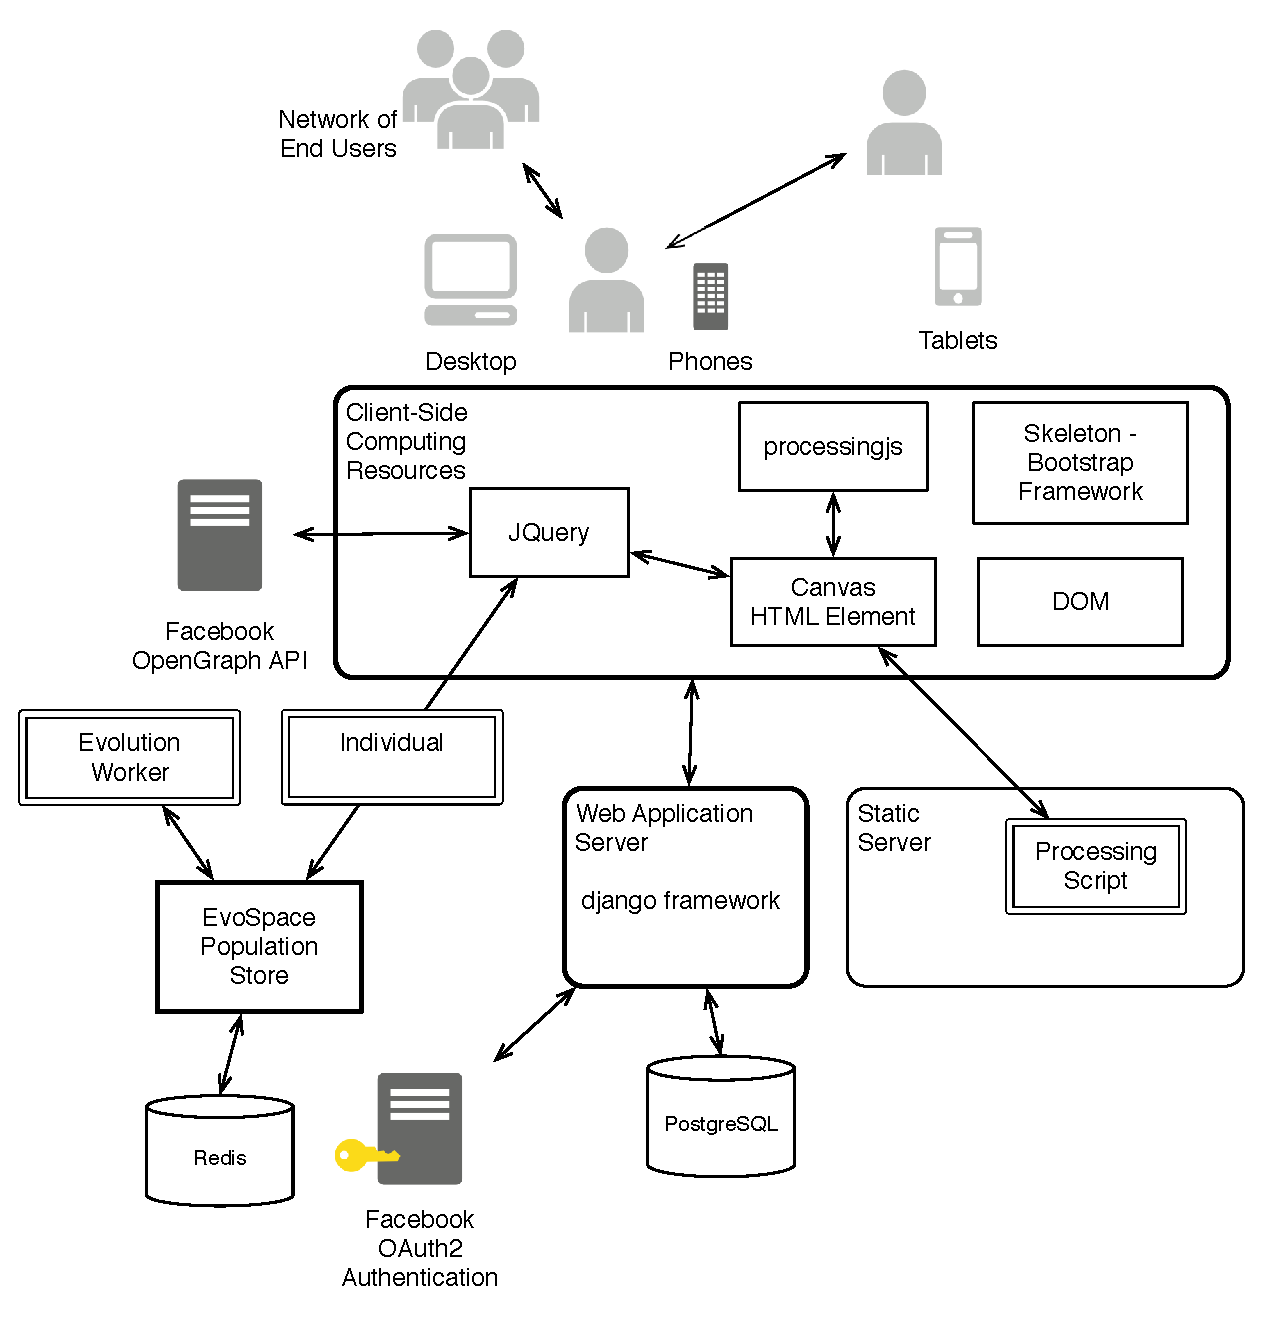
\includegraphics[width=4in]{Architecture.eps}
    \caption{Main components of EvoSpace-i.}
    \label{fig:arch}
\end{figure*}

\section{Architecture}
The goal of this work is to develop an open source framework for Web and Cloud-based C-IEA systems, using current web standards and libraries for mobile devices.
Developers of C-IEA applications are liberated from the need to design and program a platform for distributed user collaboration.
Only three components of the framework  must to be defined for each
application (marked with double lines in Figure \ref{fig:arch}), namely: an \emph{individual} representation; a \emph{processing script} that renders each individual; and a \emph{worker} script that encodes the evolutionary operators will need to be defined according to the representation and problem domain.
However, in future versions of the framework much of this work could be predefined, but also left open for advanced users to change as they require.
What the framework offers for free is: a central repository for the population implemented as an EvoSpace service; a Web Application script implemented using Django, a mature full stack Web Framework with a BSD license developed in Python.


The main components of the EvoSpace-i are shown in Figure~\ref{fig:arch}. The Interactive part is a Django \cite{django} web-based application, together with a client-side component implemented using JQuery and processingjs Javascript libraries. This application shows users a number of multimedia objects rendered in HTML5 Canvas elements. These multimedia objects are the phenotypes of individuals drawn from the Evospace population store. Evospace is responsible for storing and retrieving the data of each individual. An Evolution Worker is responsible for generating new individuals from a sample taken from EvoSpace. The evolution process is decoupled from the interactive application; thous giving IEC designers the opportunity to define their own variations of the algorithm. In the following sections each component is described in detail, staring with the population store Evospace, and then the Interactive and Collaborative components.



\section{Evospace Interactive Evolution}
In this section, the components needed to enable the interaction between users and individuals are presented. EvoSpace is presented first, then the rendering and representation of individuals. Finally, the assignment of fitness to individuals and the current breeding process is described.


\subsection{EvoSpace} % debería ser EvoSpace-i - JJ
The EvoSpace model is presented in detail in \cite{EvoSpace}, only
brief description of the functionality related to this work is given
next.  EvoSpace is inspired on the Linda language by Gelernter and
Carriero \cite{linda}; Linda is a model of coordination and
communication among several parallel processes operating upon objects
stored in and retrieved from a shared, virtual, associative memory
called {\em tuplespace}. In a tuplespace, tuples are read and removed by processes; once a tuple is taken, no other process can read it until it is written back. EvoSpace consists of two main components (see figure~\ref{fig:evo}):\begin{itemize}
\item the EvoSpace container
that stores the evolving population and
\item remote clients called
EvoWorkers, % ajústate a la terminología del abstract, "Evospace" +
            % "interactive" o "EvoStorage + EvoWorkers" - JJ
which execute the actual evolutionary process, while EvoSpace acts
only as a population repository.

\end{itemize}
Figure~\ref{fig:evo} illustrates the main components and dataflow within EvoSpace.
In a basic configuration, EvoWorkers take a random population sample from EvoSpace, 
and use it as the initial population for a local EA
executed on the client machine. After a certain number of local generations, the
evolved population is returned to EvoSpace to replace the sample.
When taken by an EvoWorker,
individuals  remain in a phantom state until their sample is
returned. If an EvoWorker does not returns a sample in a certain
amount of time, for instance because of a lost connection; individuals
are re-spawned (re-inserted) by the ReInsertionManager. Similar to
video games in which characters once killed are re-spawned after a
certain time. This can also happen when the EvoSpace container starves
or the population size is below some threshold. 

For this version of EvoSpace-i, a new type of Worker is needed: Human users. Users are responsible for evaluating the quality of individuals, the process is depicted in Figure~\ref{fig:evoInteractive}: (i) first a random sample of six individuals are taken from EvoSpace, (ii) the chromosome of each individual parameterizes a Processing script, that renders to the user, (iii) users select those individuals they like, this is stored in each individual's data, (iv) finally the sample is returned to EvoSpace. The fitness assigned to each individual can depend on the ratings given by a certain number of users. In this case the EvoWorker process is replaced  by an \texttt{Evolve()} method, that is executed after a certain number of samples have been returned.
Unlike the normal operation of EvoSpace, when a user takes a sample of individuals, these are returned with their identity unchanged, other than the rating added by the current user. The internal representation of individuals is presented next.

\subsection{Individuals} % Por qué paragraph y no subsection? Además,
                         % tiene dos puntos - JJ
As stated above, the objects stored in EvoSpace are individuals in an EA.
Explicitly, individuals are stored as \emph{dictionaries}, an abstract data type that represents a collection of unique keys and values with a one to one association. In this case, keys represent specific properties of each object and the values can be of different types, such as
numbers, strings, lists, tuples or other dictionaries.
In the current implementation, individuals are described by the following basic fields.
An \textbf{id} string that represents a unique identifier for each object.
A \textbf{chromosome} string, which depends on the EA and the representation used.
The \textbf{fitness} dictionary for each individual; In EvoSpace-i it stores pairs of user's ids and timestamp values, which represent that a user has rated the individual with a like. Currently a user can rate more than one time each individual.
The \textbf{views} The number of times the individual has been presented to a user. If a user has seen an individual and  did not assigned it a like, this can be used as a probable not-like rating.
A \textbf{parents} dictionary with identifiers of the individual(s) from which it was produced.
Finally, a \textbf{GeneticOperator}  string that specifies the operator that produced it.


Individuals are stored in-memory, using the Redis key-value database. Redis was chosen over a SQL-based management system, or other non-SQL alternatives, because it provides a hash based implementation of sets and queues which are natural data structures for the EvoSpace model. For example, selecting a random key from a set has a complexity of O(1). The logic of EvoSpace is implemented as a python module exposed by the same Django framework used by the web-based application. The EvoSpace web service interacts is called directly by a JQuery script running in the client-side. This is done by a JQuery ajax request, and using the  JSON-RPC protocol.  The EvoSpace module is available with a Simplified BSD License from \url{https://github.com/evoWeb/EvoSpace}.  The components required for the interaction between individuals and users are presented next.

\begin{figure}[!t]
    \centering
        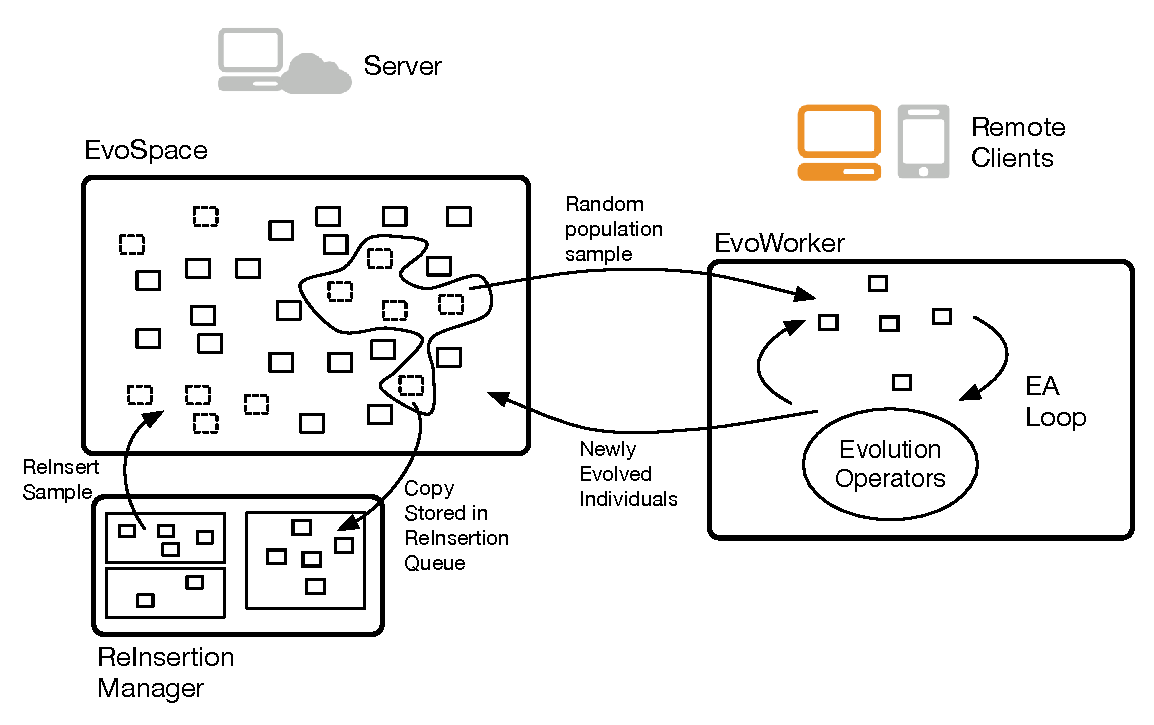
\includegraphics[width=3.3in]{evospaceExample.eps}
    \caption{Main components and dataflow within EvoSpace.}
    \label{fig:evo}
\end{figure}



\begin{figure}[!t]
    \centering
        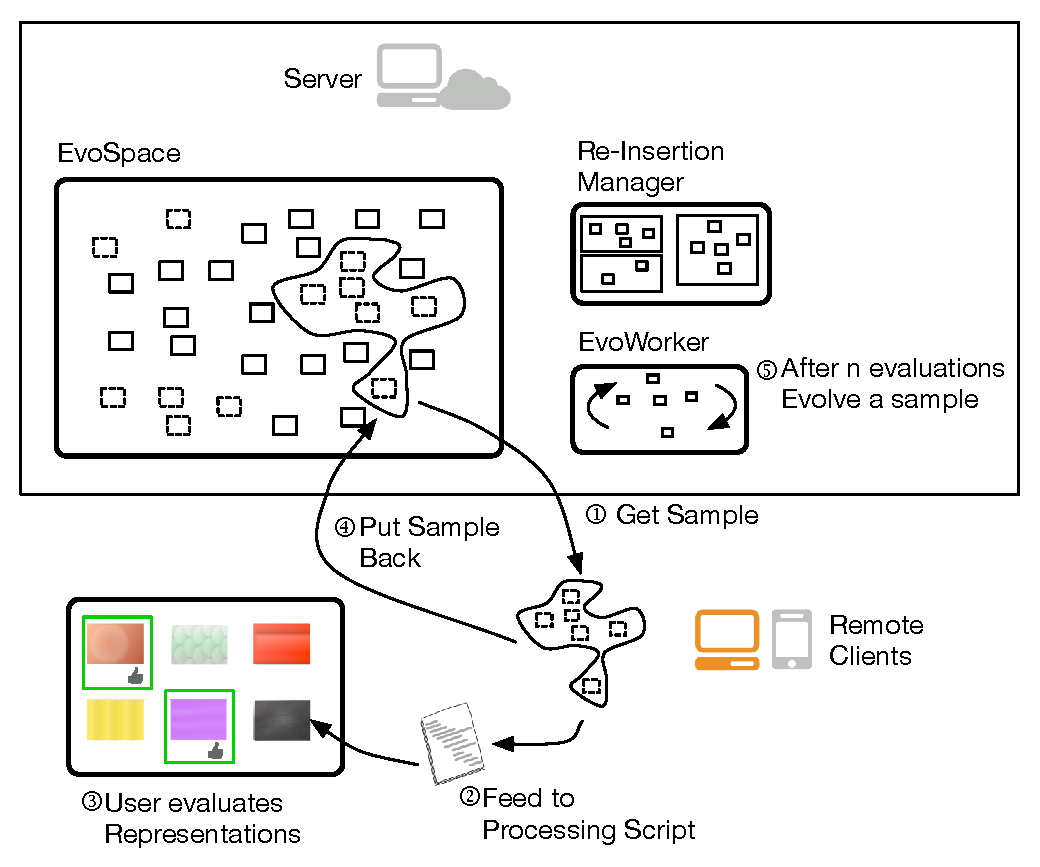
\includegraphics[width=3in]{evospaceInteractive.eps}
    \caption{Evaluation process in EvoSpace-i.}
    \label{fig:evoInteractive}
\end{figure}


\subsection{Processing Scripts}
Processing is a programming language and development environment initially created to serve as a software sketchbook and as a tool to teach fundamentals
of computer programming within a visual context.
Currently is used by artists, designers, architects, and researchers for visualization applications, games and interactive animations projects \cite{Reas:2007wp}.
Processing is a subset of Java directed to novice programmers and generative artists \cite{Pearson:2011ti}, which are the intended users of the EvoSpace-i framework.
As a complement there is a javascript library \emph{processingjs} that allows Processing scripts to be run by any HTML5 compatible browser.
Processing scripts are responsible of rendering individuals which can involve animations, sound or even interactive artifacts.
Before calling the \texttt{draw()} method of the processing script a local array of parameters are replaced with those of each individual's chromosome.
Each individual's script has its own Canvas entity; defined by the HTML5 standard, as an element that provides scripts with a resolution-dependent bitmap canvas which can be used for rendering graphics on the fly.
Although the combination of an HTML5 Canvas element and a Processing script is supported by default, other combinations could be used.
For instance, images, embedded audio, or other libraries capable of drawing in the Canvas.
Also, a fallback implementation must be considered for applications intended for non-HTML5 capable browsers.

To create a new C-IEC application, the  rendering script must be defined, and its parameters encoded as a chromosome.


\subsection{Fitness}
As stated before, the assignment of the fitness for each individual takes into account the evaluation given by several users. Initially in EvoSpace-i users can only give positive evaluations explicitly when they select an individual, giving it a rating of \emph{Like}.
When a user evaluates a sample of individuals, some (or all) of them will not receive a like, in each case the \texttt{views} property will be incremented by 1. For instance, if an individual has a high number of views with with only two likes, he considered to be  worse than an individual with two views and two likes. The ratio $Likes/Views$ is more informative, but it does not distinguish between an individual with many views and another with only
one view if they both have zero likes; also views must be >=1 to avoid dividing by zero. Fitness, therefore, it is proposed to be given by $(Likes+1)/(Views+1)$. As a future work more options can be defined, for instance taking into account the number of ``shares'' or the times an individual has been stored in a collection.

\subsection{Breeding Process}

Once individuals have been evaluated by a minimum number of users, these can participate in the breeding process. As the genetic operators of the evolution process, will depend of the particular application; this algorithm must be implemented in python. Python libraries as DEAP or PyEvolve can be used for this purpose. Both examples presented in this work were implemented using only the NumPy library for array operations. As this process is executed in the server, the communication with EvoSpace-Redis is directly through a library. Only clients connect to the Web Service. There are a few additional parameters that are used for the \texttt{Evolve()} method: \texttt{EVOLUTION-INTERVAL} indicates the number of that must returned to trigger an \texttt{Evolve()} call; the  \texttt{SAMPLE-SIZE} parameter indicates how many individuals are taken from EvoSpace to participate in the Evolution, \texttt{MINIMUM-VIEWS} is the minimum views needed for each individual to participate in the breeding process.

\section{Collaboration}
Using their Facebook account, users can collaborate with their Facebook friends, sharing those individuals they like, or taking individual from the collections of friends, as an introduction to this section de general user experience is described next.

\subsection{User Interface.}
Users interact with the web interface depicted in Figure \ref{fig:web}, which is composed of five elements.
First, at the top left corner user login and authentication.
Users can login with their Facebook account or participate as anonymous users.
Second, if a user chooses to login a list of Facebook friends that have also linked their account with the C-IEA application is presented on the left, to encourage users to interact with the system. The third element is a central \emph{ Wall } area, where a population sample of $n$ individuals is shown to the user.
These are $n$ random individuals taken from the EvoSpace server.
Here, the user can interact with the system in two ways.
He can click on the individuals he prefers, a clicked image is highlighted and this counts as a ``like'' for the individual.
Additionally, a user can choose to add an image to one of their \emph{Collections}.
A collection is a special directory to store individuals a user prefers and wishes to save. After the user finishes interacting with the current crop of individuals on the Wall, he can choose to retrieve a new sample from EvoSpace.
This is done with the fourth element of the interface, located at the top of the screen, the \emph{GetMore} button.
The button returns the current group of individuals to EvoSpace, and brings back a new one.
Each time a user performs a \emph{GetMore} click, it increments the number of samples returned, and this could  trigger a server-side \emph{Evolve()} method. The fifth element of the interface is shown at the bottom left corner, the \emph{Collections} section.
The user can create several collections, to group and organize his favorite artifacts.
Moreover, a user can browse the content of each collection and from there share images through the social network.
When a user browses over an individual a detail pane shows how many users have liked the individual.
The pane also includes a link to the individual's details, the parents, genetic operators that created it, and genealogy information.


\begin{figure}[!t]
    \centering
        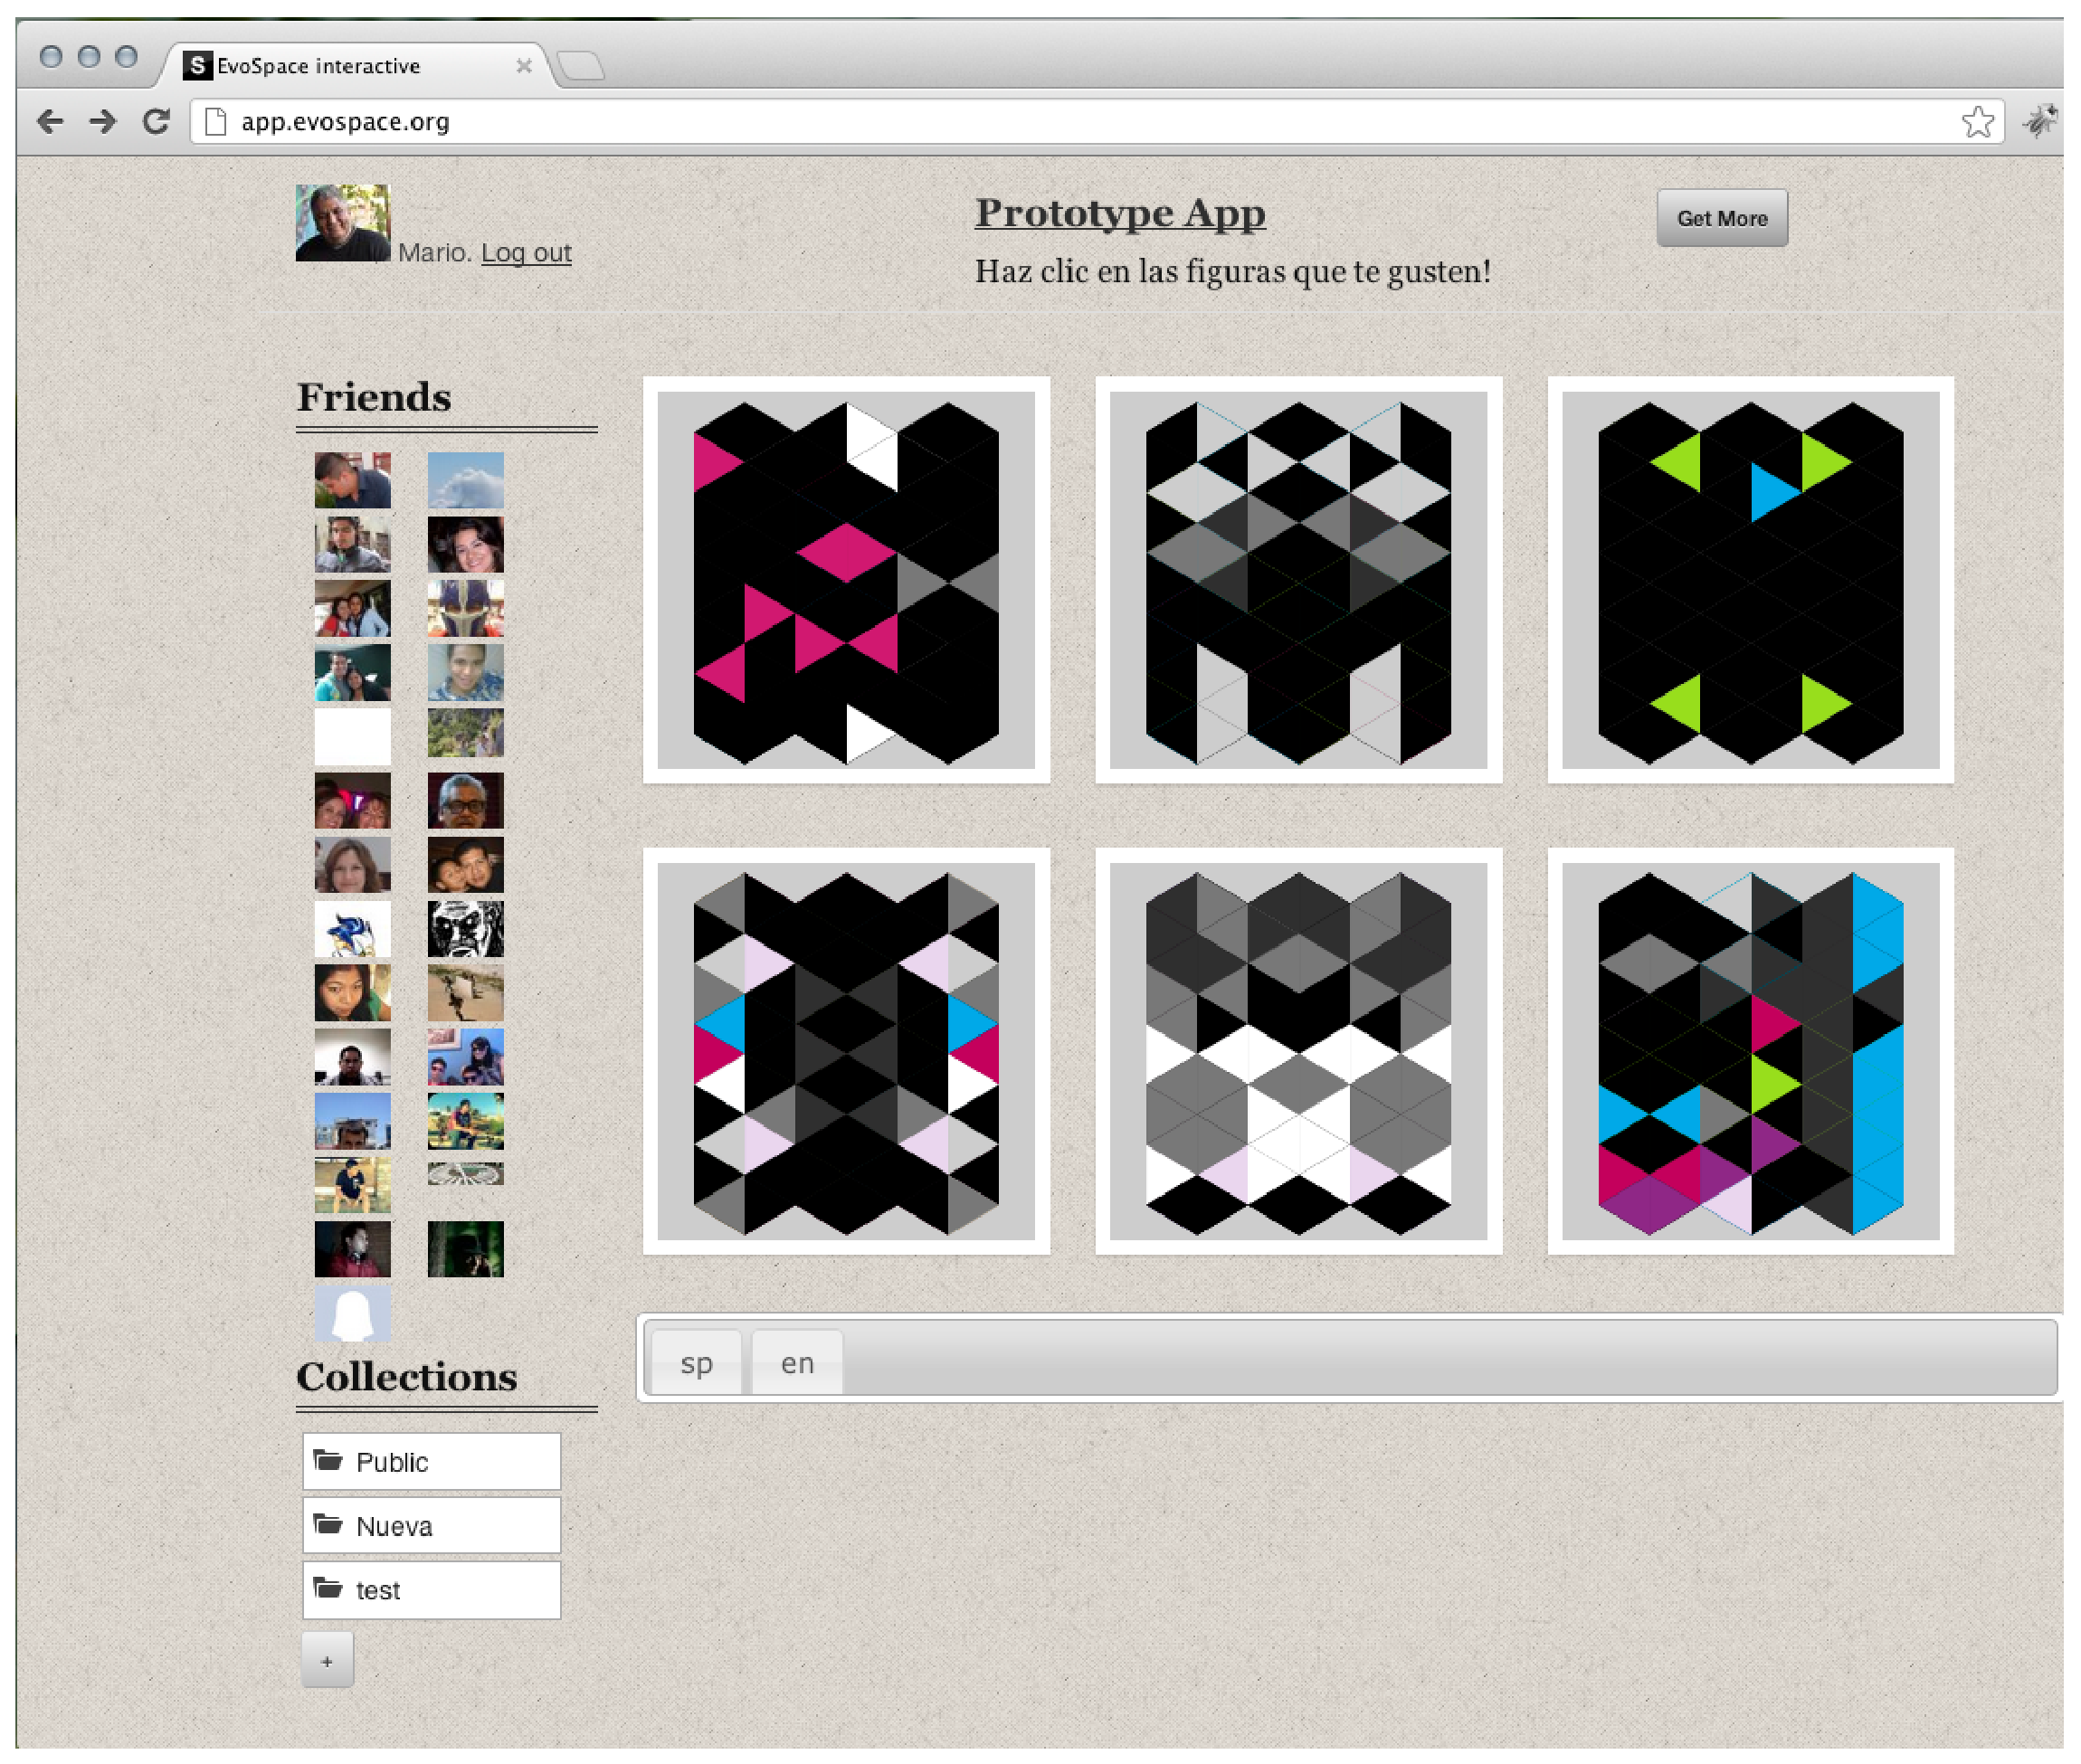
\includegraphics[width=3in]{EvoApp.eps}
    \caption{Current user interface of EvoSpace-i.}
    \label{fig:web}
\end{figure}

\subsection{Facebook API and OAuth 2.0}
Applications developed with the EvoSpace-i framework must be defined as Facebook Web Applications. Other social networks are going to be enabled in further versions of the framework; but initially Facebook was selected as a Social Network platform for the following reasons:
\begin{itemize}
	\item Popularity. Facebook is currently the social network with more active users, with more than 1 billion.

	\item Applications. Facebook applications are also common, popular applications like Youtube, Pinterest, Netflix, XBOX Live and Spotify allow users to share their activities.	
\end{itemize}
In order to enable the application's collaborative functionality, end-users must be authenticated with their Facebook account. This is done using the OAuth2.0 protocol \cite{hammer2011oauth}. The OAuth 2.0 login flow generates an access token, which you can use to make API calls on behalf of a user. As part of this flow, users also give certain permissions to the application, so it can access their private data. Currently the framework uses the most basic permission, having access only to their public profile and list of friends. The public profile includes their profile picture, username, gender and locale. An important information is the list of friends, that includes which friends also have the application installed.

\subsection{Django Framework Application}
The Django web development framework \cite{django}, is a set of Python libraries, that provide high-level abstractions of common Web development patterns. In Django a web application consists of different python scripts following a Model-View-Controller (MVC) design pattern. Using a separation of concerns design principle, the application logic is separated in mainly in four scripts:
\begin{itemize}
	\item The \texttt{models.py} script contains a class based description of the database schema. These classes are Object-Relational mappers with methods to create, retrieve, update, and delete records in your database using Python code instead of SQL.
	\item The \texttt{views.py} file contains the business logic for each web page defined as special  ``View'' functions. These functions receive as parameters and http request data, do operations on the model (database) , and return the data to feed HTML generator templates.
	\item The \texttt{urls.py} file specifies which view is called for a given URL pattern.
    \item Various HTML template files that describes the design of the page.
    \item \texttt{settings.py} file where the configuration of the project is stored.
\end{itemize}

In Django, a project can be an aggregation of multiple reusable applications, each incorporating a particular functionality. Each application has its own model, and views. For EvoSpace-i the database model is presented in Figure~\ref{datamodel}. There is a many to one relationship between facebook sessions and users, this is because sessions and access tokens can expire. The database is stored in a PostgreSQL database system. Individuals are not stored in this database, they are stored in a Redis server as JSON text. The model for individual is presented in Figure~\ref{redisModel}

\begin{figure}[!t]
    \centering
        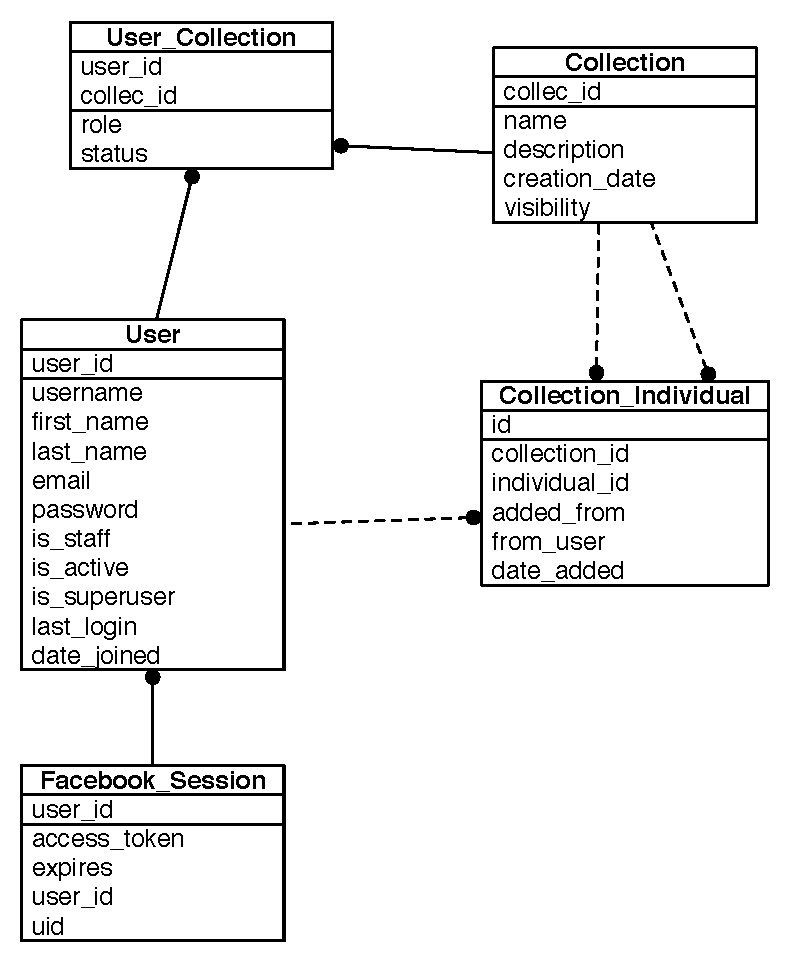
\includegraphics[width=3in]{datamodel.eps}
    \caption{Django data model for the Interactive application.}
    \label{datamodel}
\end{figure}

\begin{figure}[!t]
    \centering
        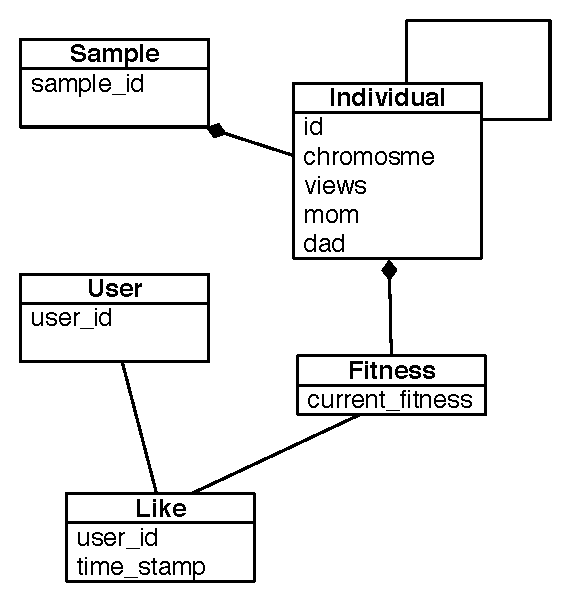
\includegraphics[width=2.3in]{redisModel.eps}
    \caption{Data model of individuals.}
    \label{redisModel}
\end{figure}

The main view functions for the application are:

\begin{description}

\item[\texttt{evospace()}] This function receives JSON-RPC requests from JQuery code in the client. Main methods are \texttt{getSample() } and \texttt{putSample()}.
\item[\texttt{home()}] This view is for the main page, if the user is authenticated the list of friends and profile data is retrieved.
\item [\texttt{individual\_view()}] This view function returns the details of Individuals.
\item [\texttt{facebook\_login()}] Initializes the OAuth 2.0 flow. The facebook\_get\_login is also related.
\item [\texttt{dashboard()}] Returns a JQuery dashboard page, for administration of EvoSpace.
\end{description}


Client-side scripting is used extensibly by the framework. As mentioned earlier, JQuery is used to implement the evaluation of individuals as shown earlier in Figure~\ref{fig:evoInteractive}, sending \texttt{getSample()} and \texttt{putSample()} requests.  Also the Javascript library processingjs is used to render each individual in its corresponding HTML5 Canvas element. Other controls such as Modal Windows, Lists, Buttons are also implemented using JQuery-UI library.

\subsection{Collections}
An important feature of the framework, is that authenticated users can create collections where they can store individuals. These collections can be private or public. Public collections can be visited by Facebook friends and if they wish, they can store individuals to their own collections. In future versions, users could also publish individuals to their Facebook Timeline or Photo Albums. Giving a sense of ownership (or in future versions authorship) to users, could be considered as a reward to their effort. This could also increase the voluntary participation of users. Information about how an individual is stored and shared, could be considered in the assignment of fitness. This way sharing can be part of the evolution. Collections are implemented as part of the web application, the database model is presented in Figure~\ref{datamodel}, there is a many to many relationship between users and collections, this way there can be shared collections, this is not yet implemented in the current version.  A collection can have many individuals, if the individual comes from another collection there is a relation with that collection. 

\section{Example Applications}
As a proof of concept a C-EIA application was implemented with the EvoSpace-i framework, this application is detailed in \cite{Musart}. The application is called \emph{Shapes}. In \emph{Shapes}, individuals represent a two dimensional 11 by 6 array of equilateral triangles, these arrays where inspired by Op-Art style paintings.
Each triangle has a color drawn from a twelve color palette.
The array is represented by a 66 element chromosome vector $\mathbf{v}=(v_1,..v_{66})$, with $v_i \in \{ 1,2,..11 \}$.
The background of the painting is Light Gray, this can give the effect of a missing triangle when it has the same color.
A processing script is used to render a static version of the image.
The breeding process uses tournament selection of size 6 to select two individuals from EvoSpace,
and generates two offspring.
The offspring replace the worst individuals from both tournament groups.
Crossover operators are used with crossover rate of 1, these are vertical and horizontal one-point crossovers.
Several mutations are used with a mutation rate of 0.3, these are:
(1) single \emph{point mutation}; (2) vertical and horizontal \emph{mirrors} at a random point;
(3) \emph{shuffle} that gives a new permutation of the chromosome.
In nearly two weeks of operation, there is a total of 70 active users, users who gave permissions to the \emph{Shapes} application and haven't
removed it from their Facebook account.
Facebook dashboard reports that 74 percent of users accepted the permission request to use their credentials to login onto \emph{Shapes}.
Participation of anonymous users was permitted, but their number was not recorded.
Basic instructions we're shown in the landing page, but part of the functionality was left to be explored by users.
An auto-increment id was assigned to each individual, after two weeks the highest id number is 8379.
A total of 17449 samples were taken from the EvoSpace server after the two week trial. A sample of artistic artifacts in a collection is depicted in Figure \ref{fig:collection}.




Another example application is \emph{Fireworks}. The goal of the Fireworks C-IEA is to evolve artistic animations of particle swarms in 3D. The animations are based on the open-source Processing script developed by Claudio Gonzales called Galactic Dust available at http://www.openprocessing.org/sketch/8062,
licensed under Creative Commons Attribution-Share Alike 3.0 and GNU GPL license. The Galactic Dust script presents a virtual 3D canvas where a set of N particles can move
about. In the original version of the script the particles are
randomly positioned within the 3D canvas (or placed in an
a priori pattern) and remain static. Then, when the user leftclicks
on a point within the canvas this specifies the position
of a gravitational point P on the canvas and produces an
attractive force on all of the particles towards P, proportional
to their distance to P and mass which is also specified initially.
Similarly, when a user right-clicks on the canvas a repulsive
force is produced. Moreover, the particles continuously change
color using small random steps and the user can toggle a
tracing effect on or off, in which each particle leaves a visual
trail of its movements that gradually disappears with time.
The Galactic Dust script is the inspiration and basis for
the artistic animations evolved by the Fireworks application.
In particular, the goal of Fireworks is to begin with randomly
placed particles and to evolve a pattern of movements and
behaviors, searching for interesting visual animations. These
animations are similar to popular screensavers or background
visualizations for music players, however the authors feel that
an illustrative description is to say that they resemble elaborate
fireworks displays, thus the name. 

The chromosome of each individual
is encoded as a variable-length list. Each element,
or gene, of the chromosome represents one of five basic
operations, these are: $Attract_{flag}$, $Move_{flag}$, $Trace_{flag}$,
$ForwardX_{flag}$, $ForwardY_{flag}$ and $Step_{m}$. The first four
instructions are toggle operations for different script parameters
that determine the characteristics of particle movements.
$Attract_{flag}$ instructs the script to toggle between attraction
or repulsion towards P. $Move_{flag}$ toggles between particle
movement or particle deceleration at each frame of the animation.
$Trace_{flag}$ determines if particle movement will produce
tracing or if it will not. $ForwardX_{flag}$ and $ForwardY_{flag}$
flags determines the orientation of particle movements in the
horizontal and vertical axis respectively. Finally, the $Step_{m}$
function determines the magnitude of step movements in each
direction given by m pixels, with a random decision uniformly
chooses from $u \in [1, 13]$.


Currently, the Fireworks applications has been
evolving individuals for over three weeks, progressively generating
novel animations. In general, it is clear that the genetic
representation and evaluation criteria has allowed the algorithm
to progressively incorporate the preferences of several users.
There is no time-table to halt the open-ended evolutionary
process, and the system is expected to run for at least one
more month. It is now possible to access the application and
interact with it at http://app.evospace.org/. It is important to
point out that the Processing scripts evolved in this work
are computationally costly, and push browser resources to the
limit. Only the Chrome web browser offers an acceptable
frame rate, using 200 swarm particles within each animation
with canvas elements of 200 by 200 pixels in size.Figure~\ref{fig:fireworks}
shows a series of frames from a singled evolved animation.
\begin{figure}[t]
    \centering
        \includegraphics[width=3in]{collection.eps}
    \caption{Artistic artifacts in a collection }
    \label{fig:collection}
\end{figure}


\begin{figure}[t]
    \centering
        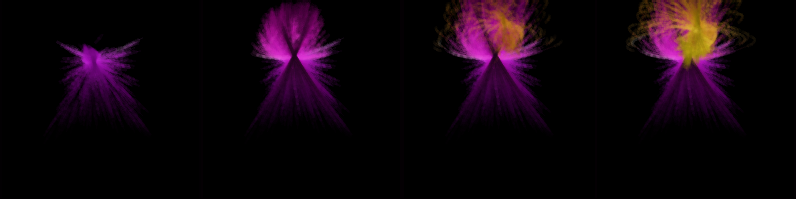
\includegraphics[width=3in]{fireworks.eps}
    \caption{Sample frames of of an evolved animation. }
    \label{fig:fireworks}
\end{figure}

\section{Conclusions}
Initial results are encouraging, the EvoSpace-i framework was successfully used to deploy a C-IEA that users accepted and used to design artistic artifacts.
Since the system integrates with a popular social network, the framework promotes the collaborative evolution of artistic memes,
leveraging the insights of multiple users in a parallel and asynchronous manner. The platform enables the collaborative assignment of fitness and provides researchers with relevant contextual information about the process, that can be considered not only in the evaluation step, but also by the system as a whole, allowing a better understanding of user behavior and preferences.
Moreover, through the use of the Processing language, and easy to develop representation of artistic artifacts is possible,
the possibilities of which were not yet pushed to the limit by the simple Shapes application, the main topic of future work and research. Nonetheless, the paper presents the first attempt to build a tool that facilitates the development and deployment of C-IEA for evolutionary art.


%\end{document}  % This is where a 'short' article might terminate

%ACKNOWLEDGMENTS are optional
\section{Acknowledgments}
This work is supported by ***

%This work is supported by projects 4616.12-P and 4617.12-P awarded by DEGEST-ProIFOPEP (Mexico), TIN2011-28627-C04-03 and -02 (ANYSELF), awarded by the Spanish Ministry of Science and Innovation, P08-TIC-03903 (EvOrq) awarded by the Andalusian Regional Government, project 83 (CANUBE) awarded by the CEI-BioTIC UGR
%(\url{http://biotic.ugr.es}) and CONACYT (Mexico) Basic Science Research Project No. 178323 and DGEST (Mexico) Research Project No. TIJ-ING-2012-110.

%
% The following two commands are all you need in the
% initial runs of your .tex file to
% produce the bibliography for the citations in your paper.
\bibliographystyle{abbrv}
\bibliography{evospace-i}  % sigproc.bib is the name of the Bibliography in this case
% You must have a proper ".bib" file
%  and remember to run:
% latex bibtex latex latex
% to resolve all references
%
% ACM needs 'a single self-contained file'!
%
%APPENDICES are optional
%\balancecolumns



\end{document}
